
\thispagestyle{empty}

\chapter{Multisensory processing in spatial orientation:\\An inverse probabilistic approach}
\chaptermark{}
\label{p1}

\newpage

\small {\bf Abstract} Most evidence that the brain uses Bayesian inference to integrate noisy sensory signals optimally has been obtained by showing that the noise levels in each modality separately can predict performance in combined conditions. Such a forward approach is difficult to implement when the various signals cannot be measured in isolation, as in spatial orientation, which involves the processing of visual, somatosensory, and vestibular cues. Instead, we applied an inverse probabilistic approach, based on optimal observer theory. Our goal was to investigate whether the perceptual differences found when probing two different states -- body-in-space and head-in-space orientation -- can be reconciled by a shared scheme using all available sensory signals. Using a psychometric approach, seven human subjects were tested on two orientation estimates at tilts \textless 120\textdegree: perception of body tilt [subjective body tilt (SBT)] and perception of visual vertical [subjective visual vertical (SVV)]. In all subjects, the SBT was more accurate than the SVV, which showed substantial systematic errors for tilt angles beyond 60\textdegree. Variability increased with tilt angle in both tasks, but was consistently lower in the SVV. The sensory integration model fitted both datasets very nicely. A further experiment, in which supine subjects judged their head orientation relative to the body, independently confirmed the predicted head-on-body noise by the model. Model predictions based on the derived noise properties from the various modalities were also consistent with previously published deficits in vestibular and somatosensory patients. We conclude that Bayesian computations can account for the typical differences in spatial orientation judgments associated with different task requirements.

\vfill

\noindent\underline{ \hspace{4cm} }

\noindent This chapter has been published as \newline
\noindent {\bf Clemens, I.A.H.}, De Vrijer, M., Selen, L.P.J., Van Gisbergen, J.A.M. and Medendorp, W.P. \citeyear{clemens2011}. Multisensory processing in spatial orientation: An inverse probabilistic approach. \emph{Journal of Neuroscience}, 31(14): 5365-5377. \newline
%\noindent Authors Clemens and De Vrijer contributed equally to this work.

\newpage

%%%%%%%%%
% Intro %
%%%%%%%%%

\section{Introduction}

To infer the current state of the body in space, the brain must rely on noisy sensory inputs. Thus, a degree of uncertainty in the reconstructed physical state is unavoidable. However, according to the rules of Bayesian inference, perceptual uncertainty can be reduced by combining overlapping information from different sensory modalities, weighting each signal in proportion to its reliability \cite{knill2004,kording2004,angelaki2008}. For example, psychophysical studies have shown that human observers behave optimally when integrating visual--proprioceptive \cite{vanbeers1999}, visual--haptic \cite{ernst2002}, or visual--auditory \cite{alais2004} cues. In these studies, the approach was to estimate noise levels of the two sensory modalities in separate unimodal experiments that were then used to predict performance in the bimodal case. Unfortunately, such a forward approach is difficult to implement when the involved sensory modalities cannot be studied in isolation, as in spatial orientation, which involves visual, somatosensory, and vestibular cues. Here the visual contribution can be eliminated easily, but to test whether somatosensory and vestibular cues are combined optimally, one cannot simply ``switch off'' one system to assess the noise level of the other. 

Instead, we took optimality as a starting point and implemented an inverse probabilistic approach to deduce noise levels of the various individual sensors. We probed two spatial orientation estimates---body-in-space and head-in-space orientation--- which, according to optimal theory, will use all available sensory signals that can be obtained by various reference frame transformations. This transformation and integration scheme, shown in \figref{p1:fig1}, involves at least three sensory systems: (1) head sensors, supplying information about the orientation of the head with respect to gravity (vestibular system); (2) body sensors, providing an estimate of the orientation of the body in space (``somatic graviceptors'') \cite{mittelstaedt1997}; and (3) neck sensors, providing an estimate of the angle between head and body (neck proprioceptors). 

\begin{figure}
    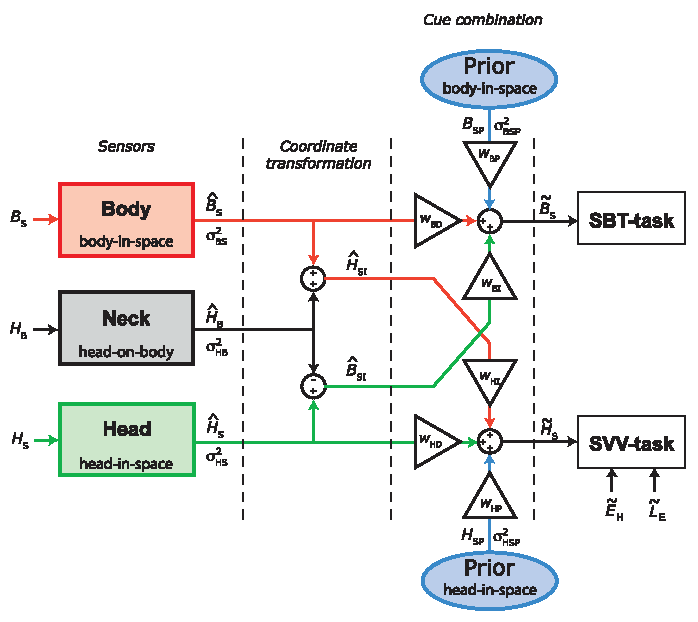
\includegraphics[width=0.75\textwidth]{src/paper1/figure1.pdf}
    
    \caption{Schematic representation of the sensory integration model. Sensory signals, denoted by a hat symbol (\textasciicircum), are assumed to be calibrated accurately, but contaminated by Gaussian noise. Optimal estimates are denoted by a tilde (\textasciitilde). Body sensors, neck sensors, and otoliths provide information about orientation of body in space ($B_S$), head on body ($H_B$), and head in space ($H_S$), respectively. Neck signal ($\hat{H}_B$) is used for a reference frame transformation of otolith information into a body-in-space signal ($\hat{H}_S - \hat{H}_B = \hat{B}_{SI}$), and for a transformation of body-tilt information into a head-in-space signal ($\hat{B}_S + \hat{H}_B = \hat{H}_{SI}$). For an optimal estimate of body-in-space orientation, $\tilde{B}_S$ (SBT task), the model combines the body-sensor signal ($\hat{B}_S$, red pathway) with a reference-frame-transformed otolith signal ($\hat{B}_{SI}$, green pathway). Relative contributions of the two pathways ($w_{BD}$ and $w_{BI}$) depend on their relative precision (\eqnref{p1:eqn2}). The scheme shows a symmetrical arrangement with two priors, but there is ample reason to believe that their effects are not identical. The simplest explanation of current and previous SBT data (see \nameref{p1:sec:methods}, \nameref{p1:sec:sbt_computation}) indicates that the associated prior in this task is uniform, which implies that $w_{BP}$ can be ignored. In the SVV task, an optimal estimate of head-in-space ($\tilde{H}_S$) is obtained by integration of otolith information ($\hat{H}_S$, green pathway), reference-frame-transformed information from body sensors ($\hat{H}_{SI}$, red pathway), and a significant contribution from prior information ($H_{SP}$, blue pathway). Relative weights are denoted by $w_{HD}$, $w_{HI}$, and $w_{HP}$, respectively. Estimate of line-in-space orientation is obtained by combining $\tilde{H}_S$ and estimates of eye-in-head ($\tilde{E}_H$) and line-on-eye ($\tilde{L}_E$) orientation. Noise variance in body sensors ($\sigma^2_{BS}$), neck sensors ($\sigma^2_{HB}$), otoliths ($\sigma^2_{HS}$), and width of prior ($\sigma^2_{HSP}$) defines their relative weights (see \nameref{p1:sec:methods}). Otolith noise may depend on tilt angle (\eqnref{p1:eqn11}). Note that the process of sensory integration, denoted here by summation of weighted sensory signals, is equivalent to multiplication of the underlying probability distributions (\eqnref[ and ]{p1:eqn2,p1:eqn6} and \nameref{p1:sec:appendix}).}
    \label{p1:fig1}
\end{figure}

In this scheme, an estimate of body orientation in space can be obtained directly from the body sensors, but also indirectly from the head-sensor signal, by subtracting the neck signal. Likewise, the estimate of head-in-space orientation can be obtained from the head sensors, but also through an indirect pathway, by combining the body-sensor signal with neck information. Importantly, as the two state estimates require different transformations, Bayesian theory predicts that the relative contribution of the sensory signals will differ as well \cite{mcguire2009}. Apart from the crucial role of sensory information, the scheme allows for the possibility that the estimates of the two orientation states can be further influenced by prior beliefs about sensory states. 

Here, we used two psychophysical tasks -- subjective body tilt (SBT) and subjective visual vertical (SVV) to quantify the two orientation estimates in a group of healthy subjects. Using an inverse probabilistic approach, we obtained stable solutions for the noise properties of the involved sensor systems. Independent measurements of neck noise confirmed the levels predicted by the model. Forward model predictions based on these noise properties were consistent with previously published deficits of bilateral vestibular and paraplegic patients, which would be difficult to explain otherwise. Our results suggest that Bayesian integration of multisensory information explains the major task-dependent features in spatial orientation perception. 


%%%%%%%%%%%
% Methods %
%%%%%%%%%%%

\section{Materials and Methods}
\label{p1:sec:methods}

\subsection{Subjects}

Seven subjects (6 male, 1 female) provided written informed consent to participate in the experiments. Ages ranged from 23 to 65 years. Subjects were free of any known vestibular or other neurological disorder and had normal or corrected-to-normal visual acuity. All subjects took part in SBT and SVV experiments (see below, \nameref{p1:sec:experiments}) and returned to the laboratory for an independent measurement of neck proprioception. Before each experiment started, subjects received careful instructions and performed a few practice runs to get used to the task. Participants never received any feedback about their performance, not even in the training trials. Each subject participated in 20 experimental sessions of {\textapprox}45 min each, yielding {\textgreater}15h recording time per participant.

\subsection{Setup}

Body tilt was controlled by a computer-controlled vestibular chair, which was configured to allow subject rotation in the roll axis. A digital position encoder measured roll position with an angular resolution of \siang{0.04}. The subject's body was tightly fixated using a five-point seat belt and adjustable shoulder and hip supports. Velcro straps restrained both legs and feet, and a padded helmet firmly fixated the head in a natural upright position for looking straight ahead. Subject-specific seat adjustments ensured that the naso-occipital axis, midway between the eyes, coincided with the roll axis of the chair. Experiments took place in complete darkness. 

\subsection{Experiments}
\label{p1:sec:experiments}

\subsubsection{SBT}
\label{p1:sec:methods_sbt}
 
The SBT experiment served to obtain a psychometric measure of each subject's accuracy and precision of body-tilt perception at five body-tilt angles: upright (\siang{0}, \SBT{0} task) and \siang{45} and \siang{90} right side and left side down (\SBT{\textpm45} task and \SBT{\textpm90} task). Negative angles indicated left side down. We applied the method of constant stimuli, using a set of 10 equidistant body-tilt angles, centred on tentative estimates of the subject's \siang{0} (SBT0), \siang{45} (\SBT{45}), \siang{-45} (\SBT{-45}), \siang{90} (\SBT{90}), and \siang{-90} (SBT-90) body-tilt percept. The latter were determined in a few pilot trials that also served to familiarise the subject with the task, without providing a reference of the five respective orientations to be tested. Relative to the test angle, we used test angle intervals of \siang{3}, \siang{4}, and \siang{4} in the \SBT{0}, \SBT{\textpm45}, and \SBT{\textpm90} tasks, respectively. Body-tilt angles were tested 14 times in random order, yielding 140 responses for each psychometric curve. 

To perform the psychophysical SBT experiments, two methodological problems had to be solved. The first relates to the number of experimental sessions that we could reasonably ask subjects to perform. We realised that returning the subject to upright for reorientation after each trial would require too large a number of experimental sessions. Our overriding concern was that starting each trial from upright would confound the \SBT{0} task in the sense that subjects could then simply notice the change in chair position. To prevent this, we always inserted a detour rotation before moving the subject to the test angle in a given trial. The detour, always to a tilt position clearly outside the psychometric test range, served to reset the subject's memory of the previous tilt position. These detour angles were chosen randomly from a range at \siang{30-40} clockwise (CW) and counterclockwise (CCW) from the presumed threshold. As an illustration, \figref{p1:fig2} shows how the subject was moved from one trial to the next in the course of an \SBT{90} experiment. Detour angles preceding each test angle were taken from the CW and the CCW detour range in equal proportions. An analysis of trial history effects indicated that detour angles did not affect the judgment in the subsequent trial ($p > 0.05$). 

%\begin{figure}
\begin{wrapfigure}{l}[5pt]{0.5\textwidth}    
    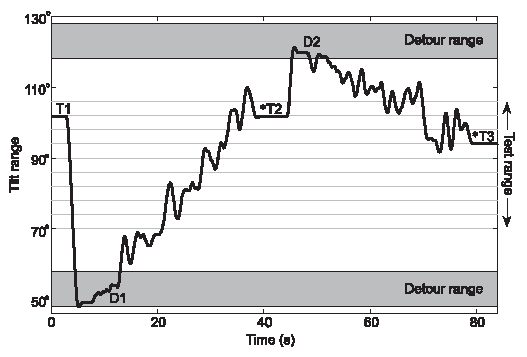
\includegraphics[width=0.5\textwidth]{src/paper1/figure2.pdf}
    
    \caption{Tilt paradigm in \SBT{90} task. T1, T2, T3, Test angles at which the subject was prompted with a beep signal (*) to indicate whether body orientation was CW or CCW from the instructed reference orientation (i.e., \siang{90} in this example). D1, D2, Detour angles randomly drawn from detour range (\siang{30-40} CW and CCW from centre of test range). Rotations from detour (D) to test (T) angle were performed in a noisy fashion (see \nameref{p1:sec:methods}, \nameref{p1:sec:methods_sbt}).}
    \label{p1:fig2}
\end{wrapfigure}

Each experimental run started in upright position with the room lights on. After the lights were turned off, subjects were first rotated at a constant angular velocity of \siang[/s]{30} to a random detour angle, outside of the test angle range, where they remained for 3 s. The chair then moved to a randomly chosen position within the test range with a very slow and noisy profile, defined by the sum of a ramp of \siang[/s]{0.4 - 2} and Gaussian white noise (bandwidth, 0 - 0.7 Hz; RMS amplitude, \siang{3.4}). Ramp speed was chosen such that the trajectory between detour angle and test angle was reached in 30 \si{\second} (\figref{p1:fig2}). These precautions were taken to enforce independent absolute tilt judgments and to deter reliance on sensed changes in tilt position that had occurred since the previous trial. Three seconds after arrival at the test angle, a beep signal prompted the subject to indicate whether body orientation was CW or CCW from the instructed reference orientation (\siang{0} in the \SBT{0} task, \siang{\textpm45} in the \SBT{\textpm45}, or \siang{\textpm90} in the \SBT{\textpm90} task), using a toggle switch. The subject was then rotated at a constant velocity to a new randomly drawn detour angle, and the above procedure was repeated. Each run, comprising seven test angles, lasted \textapprox5 min, after which the subject was rotated back to upright, and room lights were turned on. Between runs, there was a 60 s rest interval before the next run started. Each SBT task was tested in separate sessions of \textapprox45 min each, thus amounting to a total of 15 sessions per subject (i.e., \textapprox11 h of recording time).

\subsubsection{SVV}
 
The same subjects were also tested in a series of SVV experiments. Part of this dataset (four subjects) has been published previously as part of a larger dataset on visual verticality perception \cite{devrijer2009}. Data in the other three subjects were collected anew. Here we provide a brief summary of the paradigm. SVV was tested at nine roll-tilt angles, ranging from -120 to \siang{120} at \siang{30} intervals. A luminous line (angular subtend, \siang{20}), polarised with a bright dot at one end, was mounted in front of the subject. The line's rotation axis coincided with the chair rotation axis. In each experimental run, the subject was rotated from upright to the chosen test angle at a constant angular velocity of \siang[/s]{30}. After a 30 \si{\second} waiting period that allowed canal effects to subside, a luminous line was briefly flashed (20 \si{\milli\second}), and the subject indicated whether its orientation in space was CW or CCW from the perceived direction of gravity. The line orientation was selected randomly from a set of 11 line orientations. After all line orientations had been tested, the subject was rotated back to upright, and room lights were turned on. Positive and negative body-tilt angles were alternated regularly. As in the SBT experiment, we used the method of constant stimuli. The set of 11 line orientations was centred on a coarse estimate of the SVV threshold at each tilt angle. We used orientation intervals of \siang{3}, except for upright, where intervals of \siang{2} were taken. Each set of line orientations was tested in random order in 12 experimental runs, thus yielding a total of 132 responses for each psychometric curve. SVV data were collected in a total of five 45 min sessions per subject. 

\subsection{Data analysis}

CW tilt angles of the body and the luminous line were defined positive. We quantified performance, for each roll-tilt angle (5 in the SBT and 9 in the SVV) independently, by examining the proportion of CW responses as a function of body orientation (SBT) and the proportion of CCW responses as a function of line orientation with respect to the body (SVV). Psychometric data were quantified by fitting a cumulative Gaussian function (\figref{p1:fig3}): 

\begin{equation}
\label{p1:eqn1}
P(x) = \lambda + (1 - 2\lambda) \frac{1}{\sigma \sqrt{2\pi}} \int_{-\infty}^{x}{e^{-(y-\mu)^2 / 2\sigma^2}}dy,
\end{equation}
% Equation 1


in which $x$ represents body orientation in space (SBT experiment) or line orientation with respect to the body (SVV experiment). The mean of the Gaussian $\mu$ represents the subjective perception of the reference orientation in the SBT task, or the SVV compensation angle (the angle between the apparent visual vertical line and the body axis) in the SVV task. The width of the curve, $\sigma^2$, inversely related to precision, serves as a measure of the subject's variability in the SBT or SVV task. Parameter $\lambda$, representing the lapse rate, accounts for stimulus-independent errors caused by subject lapses or mistakes and was restricted to small values ($\lambda < 0.06$). Fits were performed using Matlab software (MathWorks) with the ``psignifit'' \cite{wichmann2001b} routine. 

\subsection{Sensory integration model}

To provide a theoretical framework that explains the observed responses, we designed a sensory integration model for visual verticality and body-tilt perception that assumes optimal processing of all potentially relevant sensory signals, including body, head, and neck sensors. The model links accuracy and variability in the two spatial tasks to the properties of the underlying sensors. For simplicity, the scheme is limited to SBT and SVV signal processing in darkness. 

In the scheme (\figref{p1:fig1}), we use the following conventions: physical variables are denoted by a capital with a subscript indicating the frame of reference. For example, $H_S$ represents the physical orientation of the head in space. Sensory signals and their reference-frame-transformed counterparts are denoted by a hat symbol (\textasciicircum), as in $\hat{H}_{S}$, which represents the orientation of the head in space as measured by the head-in-space sensors. The optimal estimate of a variable, obtained by integration of all available information, is indicated by a tilde (\textasciitilde), as in $\tilde{H}_S$, representing the final head-in-space estimate. 

It is assumed that all sensory signals are accurately calibrated (i.e., unbiased) but corrupted by independent Gaussian noise with a given variance ($\sigma^2$), with subscripts to indicate the sensory modality (e.g., $\sigma_{BS}^2$ represents noise variance in the body-in-space sensors). 

\subsubsection{SBT computation}
\label{p1:sec:sbt_computation}
 
To obtain an estimate of the orientation of the body in space, the brain can use ``direct'' sensory information from body sensors ($\hat{B}_S$), such as tactile receptors in the skin or so-called graviceptors in the trunk \cite{mittelstaedt1997, mittelstaedt1998, vaitl2002}. Alternatively, an ``indirect'' pathway, involving a reference frame transformation, can also provide a body-in-space estimate. For this purpose, sensory head-in-space information, provided by the otoliths, must be combined with information about head-on-body orientation, provided by proprioceptive signals from the neck ($\hat{B}_{SI} = \hat{H}_S - \hat{H}_B$). Because the sensors are contaminated by noise, the direct and indirect signals can be represented as Gaussian probability distributions with mean values of $\hat{B}_S$ and $\hat{H}_S - \hat{H}_B$, and variance levels of $\sigma_{BS}^2$ and $\sigma_{HS}^2 + \sigma_{HB}^2$, respectively. Theoretically, as shown in \figref{p1:fig1}, the brain could also use prior information about body-in-space orientation in the computation of the body-in-space estimate. The effect of including a prior on the SBT (centred on upright) would be a systematic error of underestimation at larger tilt angles. However, neither previous findings \cite{mittelstaedt1983, mast1996, jarchow1999, vanbeuzekom2001} nor the present results (\figref[ and ]{p1:fig3,p1:fig4}), showed such systematic errors across subjects. In modelling terms, this indicates a uniform (uninformative) prior, which corresponds to a weight of 0. Accordingly, a statistically optimal estimate of body-in-space orientation ($\tilde{B}_S$) is then given by the peak of the Gaussian distribution that results from the multiplication of the two distributions representing the direct and indirect sensory pathways. It follows that

\begin{equation}
\label{p1:eqn2}
\tilde{B}_S = w_{BD} \cdot \hat{B}_S + w_{BI} \cdot (\hat{H}_S - \hat{H}_B),
\end{equation}

with

\begin{equation}
\label{p1:eqn3}
w_{BD} = \frac{1/\sigma^2_{BS}}{1/(\sigma^2_{HS} + \sigma^2_{HB}) + 1/\sigma^2_{BS}}
\end{equation}

and

\begin{equation}
\label{p1:eqn4}
w_{BI} = \frac{1/(\sigma^2_{HS} + \sigma^2_{HB})}{1/(\sigma^2_{HS} + \sigma^2_{HB}) + 1/\sigma^2_{BS}}
\end{equation}

in which $w_{BD}$ and $w_{BI}$ (\figref{p1:fig1}) represent the respective weights of the direct and indirect pathways, which add up to 1 \cite{landy1995,jacobs1999,ernst2002,bays2007}. Note that the weight of each pathway depends on its reciprocal noise variance (also known as precision), so that precise signals have a stronger influence on the final estimate than noisy signals. Furthermore, because both sensory pathways are supposed to carry unbiased signals, the mean estimate of body in space in multiple trials, $\mu(\tilde{B}_S)$, will also be accurate. 

It can further be shown that the variance in $\tilde{B}_S$ in multiple trials, denoted as $\sigma^2(\tilde{B}_S)$, equals 

\begin{equation}
\label{p1:eqn5}
\sigma^2(\tilde{B}_S) = \frac{
\sigma^2_{BS} \cdot (\sigma^2_{HS} + \sigma^2_{HB})
}{
\sigma^2_{BS} + (\sigma^2_{HS} + \sigma^2_{HB})
}
\end{equation}

which implies that the final estimate has a lower variance than the signal provided by either the direct or the indirect pathway \cite{ernst2002,ernst2004}. Because we assume that sensory signals are accurate and that there is no prior information about body in space, the model predicts that there are no systematic errors in the SBT, so that $\mu(\tilde{B}_S) = B_S$. The variance in the SBT task is represented by $\sigma^2(\tilde{B}_S)$. 

\subsubsection{SVV computation}

The scheme applies a similar sensory signal processing strategy to estimate the orientation of head in space, $\tilde{H}_S$, used in the SVV. A direct estimate of head-in-space orientation is provided by the head-in-space sensors ($\hat{H}_S$), and an indirect estimate is obtained by a reference frame transformation of the body-in-space signal ($\hat{B}_S$) by adding the head-on-body estimate ($\hat{H}_B$), provided by the neck sensors ($\hat{H}_{SI} = \hat{B}_S + \hat{H}_B$). Again, direct and indirect pathway signals are represented by two Gaussian probability distributions, with mean values of $\hat{H}_S$ and $\hat{B}_S + \hat{H}_B$, respectively, and corresponding variances of $\sigma^2_{HS}$ and $\sigma^2_{BS} + \sigma^2_{HB}$. In the computation of the head-in-space estimate, to account for systematic errors \cite{macneilage2007, devrijer2008}, it is further assumed that the brain uses prior knowledge about head-in-space orientation, which entails that small head-tilt angles are considered more probable than large tilts. Mathematically, the prior is represented by a Gaussian distribution that is centred at \siang{0} head tilt ($H_{SP} = 0^\circ$) with a variance of $\sigma^2_{HSP}$. Note that, in our scheme, the head-in-space prior, which contributes to the SVV computations, does not affect the body-in-space estimate. Integration of the direct and indirect sensory pathways and prior knowledge is performed by multiplication of the three Gaussian distributions. The peak of the resulting posterior distribution represents the optimal estimate of head-in-space orientation ($\tilde{H}_S$), which is given by the following: 

% Equation 6
\begin{equation}
\label{p1:eqn6}
\tilde{H}_S = w_{HD} \cdot \hat{H}_S + w_{HI} \cdot (\hat{B}_S + \hat{H}_B) + w_{HP} \cdot H_{SP}
\end{equation}

with

% Equation 7/8
\begin{equation}
\label{p1:eqn7}
w_{HD} = \frac{1 / \sigma^2_{HS}}{1 / (\sigma^2_{BS} + \sigma^2_{HB}) + 1/\sigma^2_{HS} + 1/\sigma^2_{HSP}},
\end{equation}

\begin{equation}
\label{p1:eqn8}
w_{HI} = \frac{1 / (\sigma^2_{BS} + 1/\sigma^2_{HB})}{1 / (\sigma^2_{BS} + \sigma^2_{HB}) + 1/\sigma^2_{HS} + 1/\sigma^2_{HSP}}
\end{equation}
% Check eqn. 8 the 2nd 1/ might be a mistake

and

\begin{equation}
\label{p1:eqn9}
w_{HP} = \frac{1 / \sigma^2_{HSP}}{1 / (\sigma^2_{BS} + \sigma^2_{HB}) + 1/\sigma^2_{HS} + 1/\sigma^2_{HSP}}
\end{equation}
% Equation 9

In this equation, $w_{HD}$, $w_{HI}$, and $w_{HP}$ (which add up to one) represent the weights of the direct and indirect pathways and the prior, respectively, which are proportional to the relative precision of the sensory signals and the width of the prior. \eqnref{p1:eqn6} would result in an accurate estimate of $\tilde{H}_S$, if all three pathways were accurate by themselves. However, because the prior is centred on zero ($H_{SP} = 0\degree$), it introduces more and more bias toward upright, as head tilt increases further. Thus, optimization in terms of variance has a downside by causing underestimation of the actual head tilt. The amount of underestimation depends on the width of the prior and the reliability of the sensory inputs.

The variance in the head-in-space estimates, measured across many trials, $\sigma^2(\tilde{H}_S)$, can be derived directly from \eqnref{p1:eqn6} by applying the rules of error propagation (see \nameref{p1:sec:appendix} for complete derivation). From these calculations, it follows that 

% Equation 10
\begin{equation}
\label{p1:eqn10}
\sigma^2(\tilde{H}_{S}) = w^2_{HD} \cdot \sigma^2_{HS} + w^2_{HI} \cdot (\sigma^2_{BS} + \sigma^2_{HB}),
\end{equation}

in which the variance contributions of the direct and indirect pathways are represented by their squared weights. Although it does not appear explicitly in \eqnref{p1:eqn10}, it is important to notice that the prior has a noise-reducing effect by downscaling the sensory-related weighting terms ($w_{HD}$ and $w_{HI}$). The narrower the prior, the larger its relative weight ($w_{HP}$) and the smaller the sensory weights, because $w_{HD} + w_{HI} + w_{HP} = 1$. Thus, the effect of the head-in-space prior is twofold: it reduces the variance, but as noticed above, this occurs at the cost of a bias in the final estimate of head-in-space orientation, which becomes pronounced at large tilts (see \nameref{p1:sec:appendix} for further details). 

Previously, we have shown that to account for the typical nonlinear increase of the systematic SVV errors with tilt, the variability of the head-tilt signal in the model must increase with tilt angle \cite{devrijer2008,devrijer2009}. In line with this conclusion, decreasing effectiveness of the otoliths with increasing tilt has been suggested by various other reports \cite{schone1968,tarnutzer2009,tarnutzer2010} and may reflect the geometry of otolith organs, the nonuniform distribution of otolith afferents in the roll-plane and nonlinear firing rates \cite{tarnutzer2010}. This feature was incorporated by allowing the noise in the sensory head-tilt signal, $\sigma_{HS}$, to increase rectilinearly with tilt angle: 

% Equation 11
\begin{equation}
\label{p1:eqn11}
\sigma_{HS} = a_{HS} |H_S| + b_{HS}
\end{equation}

in which $a_{HS}$ reflects the proportional increase of noise with tilt angle and $b_{HS}$ represents the noise at $H_{S} = 0\degree$. Note that, in the data fits, parameter $a_{HS}$ was allowed to be zero, so that the present model did not force $\sigma_{HS}$ to depend on head tilt. 

To compute the SVV, the brain not only requires an estimate of head orientation in space ($\tilde{H}_S$), but also needs estimates of eye-in-head orientation ($\tilde{E}_H$) and retinal line orientation ($\tilde{L}_E$). Together, these signals determine the orientation of a visual line in space ($\tilde{L}_S$) according to $\tilde{L}_S = \tilde{H}_S + \tilde{E}_H + \tilde{L}_E$. The systematic error in the SVV experiment (${\Delta}SVV$) corresponds to the error in $\tilde{L}_S$ and is thus given by ${\Delta}SVV = {\Delta}H_S + {\Delta}E_H + {\Delta}L_E$, in which $\Delta$ denotes the bias in each estimate. For simplicity, we assumed that the visual signal representing retinal line orientation is accurate, so that ${\Delta}L_E = 0\degree$. As explained in a previous study \cite{devrijer2009}, underestimation of eye torsion causes errors in the eye-in-head estimate (${\Delta}E_H$), which can be represented by ${\Delta}E_H = -A_{OCR} \cdot \sin(\hat{H}_S$, where parameter $A_{OCR}$ denotes uncompensated ocular counterroll. Finally, the error in the head-in-space estimate is obtained by subtracting $\tilde{H}_S$ (see \eqnref{p1:eqn6}) from the actual head tilt $H_S$, which ultimately leads to the following relation for the mean SVV error, $\mu({\Delta}SVV)$, in multiple trials: 

% Equation 12
\begin{equation}
\label{p1:eqn12}
\mu({\Delta}SVV) = (1 - w_{HD} - w_{HI}) \cdot H_S - A_{OCR} \cdot \sin(H_S)
\end{equation}

In \eqnref{p1:eqn12}, the influence of the prior works through the weight factors $w_{HD}$ and $w_{HI}$. Because these weights do not add up to 1 (see above, $w_{HD} + w_{HI} = 1 - w_{HP} < 1$), the result is a systematic error in the head-in-space estimate, which becomes more pronounced at large tilt. The noise level in the eye-in-head and line-on-eye estimates is probably relatively small compared with the noise in the head-in-space estimate considering results from Vandenbussche et al. \citeyear{vandenbussche1986}, who reported just-noticeable difference levels for orientation discrimination of \siang{\textless1}. Given this low value, SVV variance is determined mainly by the variance in the latter estimate, so that $\sigma^2({\Delta}SVV) \sim \sigma^2(\tilde{H}_S)$.

\subsection{Model fitting}

The model contains seven fit parameters ($a_{HS}$, $b_{HS}$, $\sigma_{HSP}$, $\sigma_{BS}$, $\sigma_{HB}$, $A_{OCR}$, and $\lambda$) that were fitted to all data (SBT and SVV) simultaneously for each subject. As stated earlier, parameters $a_{HS}$ and $b_{HS}$ represent the increase and offset of sensory noise in the head-in-space estimate, respectively. The parameter $\sigma_{HSP}$ denotes the width of the prior distribution, reflecting a priori knowledge about head-in-space. Noise levels in the body and neck sensors are represented by parameters $\sigma_{BS}$ and $\sigma_{HB}$. Finally, the amplitude of uncompensated ocular counterroll is denoted by $A_{OCR}$. In addition to these six parameters related to sensory processing, there is a seventh parameter to account for lapses ($\lambda$). 

In addition to these ``parameters of interest'', the data were preprocessed before model fitting by applying mean correction \cite{mcguire2009}. Mean correction was performed to remove systematic errors in the SBT and the asymmetries in the SVV between CW and CCW tilt angles. Because the model is inherently left-right symmetric, it would try to account for differences in SVV bias between equal but opposite tilt angles by falsely increasing the variance. Likewise, because the model assumes that there is no bias in the SBT, it would try to explain any slight deviation from zero by excessively increasing the variance. The asymmetry in the SVV, if any, and a nonzero SBT bias, if any, are captured by fixed parameters of non-interest (n = 9) in the model fits. Thus, for the SBT data, one bias correction term was needed for each tilt angle (yielding five parameters of non-interest), and for the SVV data, one correction parameter was needed for each pair of equal but opposite tilt angles (yielding four parameters of non-interest). We emphasise that the nine parameters of non-interest are not free-fit parameters because they are not optimised by the model. So, although technically our number of free parameters amounts to a total of 16, only seven were determined by fitting the model. 

In total, the seven free parameters of the model had to account for 149 data points, spread across various tilt angles, with each data point reflecting a proportion of CW responses based on either 14 (for the SBT) or 11 (for the SVV) experimental forced-choice CW/CCW responses. We fitted the model by maximizing the likelihood of the data [maximum likelihood estimation (MLE)], in relation to the set of six model parameters ($a_{HS}$, $b_{HS}$, $\sigma_{HSP}$, $\sigma_{BS}$, $\sigma_{HB}$, and $A_{OCR}$) and lapse rate ($\lambda$). Optimal parameter values were obtained by minimizing the negative likelihood function using the Matlab function ``fmincon'' \cite{devrijer2008, mcguire2009}. Simulations confirmed that the inverse modelling approach was not sensitive to overfitting. SDs of the best-fit parameters were obtained by performing 1999 bootstrap runs. For each run, we constructed 149 data points (reflecting the size of the dataset), each of which was obtained by random sampling with replacement from the original dataset. The model was fit to this new dataset. The distribution of model parameters across all runs was used to derive the 68.2\% confidence interval of each parameter. 

We emphasise that the model fit provided an estimate of the proprioceptive variance of the neck ($\sigma_{HB}$), even though the head-on-body signal was not directly manipulated during the experiment. Nevertheless, this signal, as sensed by the neck proprioceptors, is essential to implement the reference frame transformation from the body-in-space to the head-in-space signal, and vice versa. Because the neck signal is noisy, these reference frame transformations induce neck-related noise in the original $B_S$ and $H_S$ signals, even when the head and body are aligned. Because the SBT and SVV tasks require different reference frame transformations, they depend differently on the noise properties of the three sensory systems (body and neck sensors and otoliths). By solving the inverse problem, the noise properties of the three sensory systems, as well as the other fit parameters, can be determined. Finally, we note that the inverse problem can only be solved using both tasks at multiple tilt angles; just using a single task (SVV or SBT, not both) would have made this problem intractable. 

\subsection{Model evaluation}

To assess the importance of cross-modal sensory integration, we also fitted our model without the indirect, cross-modal pathways by setting the head-on-body noise to infinity, which effectively eliminates the indirect pathways and removes one degree of freedom. To compare the maximum-likelihood estimates from the full and the reduced model, we used a log-likelihood ratio test. The test statistic is two times the difference between the negative log-likelihoods of the data, given the reduced and the full model. A $\chi^2$ test with one free parameter (the difference in degrees of freedom between the two models) is used to calculate the $p$ value \cite{dobson2001}.

Furthermore, we evaluated our mechanistic model in comparison with a pure descriptive model of the same dataset based on separate psychometric accounts, each with three free parameters, at the five SBT and nine SVV angles. We used the Bayesian information criterion (BIC) for model comparison. BIC provides a measure of the adequacy of the model fit and corrects for the number of parameters. The BIC is defined as $BIC = -2 \log(L) + k \cdot \log(n)$, in which $L$ is the total likelihood of the data given the model, $k$ the number of free parameters, and $n$ the number of data points to be explained. The number of free parameters is 42 [14 psychometric curves $\times$ 3 parameters ($\mu$, $\sigma$, and $\lambda$)] for the psychometric curves, whereas for the mechanistic Bayesian model, the number of free parameters is seven. A more appropriate model is characterised by a lower BIC value. 

%%%% ^^^ Fixme x should be cross

\subsection{Model validation: independent test of neck noise}

The SBT and SVV measurements to test the model proposed in \figref{p1:fig1} have yielded solutions for the noise properties of the involved sensor systems. To validate the model structure and the noise predictions that were obtained, we also devised an experiment that independently measured the noise in the neck sensors (head-on-body sensors), in a psychometric fashion. In this experiment, subjects were lying on a bed, in supine position, with their head fixed on a rotating platform. The platform was constructed such that it could passively rotate the head relative to the body, in the roll plane, while accounting for the shifting rotation axis in the neck vertebrae. The rotation of the platform was computer controlled, keeping the speed below \siang[/s]{0.2}, which is far below detection threshold of the canals \siang[/s]{$>0.5$}) \cite{benson1989}. In the supine condition, there is no gravity modulation of the otolith signal, so we excluded the contribution of the vestibular system in detecting head-on-body orientation and were only probing the role of the neck afferents. We applied the method of constant stimuli, using a set of 11 head angles relative to body midline. Test angles ranged from $-6\degree$ to $6\degree$. 

In complete darkness, subjects were first rotated at a constant angular velocity of \siang[/s]{$\leq15$} to a random detour angle similar to the idea shown in \figref{p1:fig2}. The head then moved to a randomly chosen position within the test range with a very slow speed (\siang[/s]{$<0.2$}) such that the test angle was reached within 20 \si{\second}. Meanwhile, auditory white noise was presented to the subjects through earphones to mask any auditory cues generated by the moving platform. After arrival at the test angle, the auditory noise was interrupted, signalling the subject to indicate whether head-on-body orientation was CW or CCW relative to the body midline, using a toggle switch. The subject was then rotated at a constant velocity to a new randomly chosen detour angle, and the above procedure was repeated. Each test angle was repeated 10 times, yielding a total number of 110 responses in each subject. Psychometric data were quantified by fitting a cumulative Gaussian function (see above, \eqnref{p1:eqn1}). The width of the curve, $\sigma^2$, inversely related to precision, serves as an independent measure of the subject's variability of the head-on-body estimate and was compared with the model prediction. 

\subsection{Model simulation of patient data}

Based on the average parameter values of the model established in normal, healthy subjects, the model was also used to make predictions about SVV and SBT performance in two patient groups: bilateral vestibular patients and patients with somatosensory loss. The model simulated SVV and SBT in these patient groups by raising the variance values of the lost signals to infinity. 


%%%%%%%%%%%
% Results %
%%%%%%%%%%%

\section{Results}

\subsection{Psychometric results}
 
The SBT experiment, performed in seven subjects, tested the accuracy and precision of SBT percepts, near upright (SBT0), at \siang{45} and \siang{90} right side down (\SBT{45} and \SBT{90}), and at \siang{45} and \siang{90} left side down (\SBT{-45} and \SBT{-90}). The same subjects also performed the SVV experiment, tested at nine roll-tilt angles, ranging from \siang{-120} to \siang{120} in \siang{30} intervals. \figref{p1:fig3} shows the results of a typical subject (S1) in both tasks. The top panels show the proportion of CW responses for the five SBT tasks, relative to the reference orientation. For an ideal observer, all psychometric functions would resemble a step centred at zero. Across the five reference orientations (\siang{0}, \siang{{\textpm}45}, or \siang{{\textpm}90}), the psychometric data indicate underestimations and overestimations of perceived body angle, but no consistent bias, which resembles previous reports \cite{mittelstaedt1983, mast1996, jarchow1999, vanbeuzekom2001} that body-tilt perception is accurate on average. We fitted psychometric curves through these data (see \nameref{p1:sec:methods}, Eq. \ref{p1:eqn1}), to obtain estimates for the mean ($\mu$), SD ($\sigma$), and lapse rate ($\lambda$). Parameter $\mu$ is a measure for the accuracy of the subject's body-tilt percept. Perceptual variability, inversely related to precision, is reflected by $\sigma^2$, whereas the lapse rate ($\lambda = 0.06$) accounts for stimulus-independent errors \cite{wichmann2001}. In all five SBT tasks, the $\mu$ values are relatively close to the veridical reference orientation (0\textdegree, 45\textdegree, or 90\textdegree), i.e., errors are \textless5\textdegree. The psychometric fits further show that variability is lower in the \SBT{0} task, with $\sigma \approx 4\degree$, than in the \SBT{\textpm45} and \SBT{\textpm90} task, where $\sigma \approx 10\degree$. 

\begin{figure}
    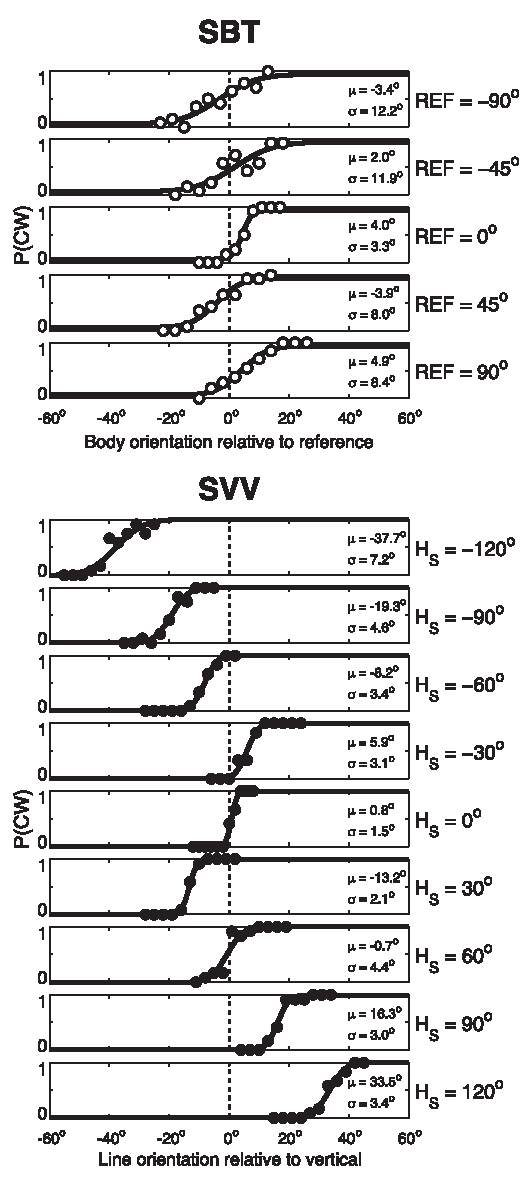
\includegraphics[width=0.5\textwidth]{src/paper1/figure3.pdf}
    
    \caption{SBT versus SVV performance in one subject (S1). Top, SBT. Proportion of CW responses is plotted against body orientation relative to the reference orientation (0 \si{\degree}, \textpm45 \si{\degree}, or \textpm90 \si{\degree}). $\mu > 0\degree$ indicates tilt underestimation. Bottom, SVV. Proportion of CW responses is plotted against line orientation relative to vertical. Solid lines, Best-fit cumulative Gaussians, typified by $\mu$ and $\sigma$.}  
    \label{p1:fig3}
\end{figure}

The bottom section of \figref{p1:fig3} illustrates the performance of the same subject in the SVV task. Each panel demonstrates how the fraction of CW responses changes as a function of line orientation relative to the perceived vertical, for each tilt angle tested. Performance is very accurate in the upright condition. For moderate body tilts, i.e., 30\textdegree, this subject shows small systematic errors, indicating that the line must be set in a direction opposite to the head tilt to be perceived vertical in space. For larger tilts ($\ge 60$), systematic errors occur with increasing tilt angle, with amplitudes up to 40 \si{\degree}, as if tilt is underestimated. This response pattern is consistent with previous literature \cite{aubert1861, udodehaes1970, mittelstaedt1983, vanbeuzekom2000}. Close scrutiny also reveals that the precision in the vertical percept deteriorates away from the upright position. 

Psychometric fits capture these observations. In the upright position, the percept of visual vertical is virtually unbiased, as indicated by a $\mu$ value of 0.8\textdegree. At large tilts, e.g., at \siang{-120} and 120\textdegree, $\mu = -37.7\degree$ and $\mu = 33.5\degree$, respectively, which means that the line must be tilted away from true vertical to be perceived as vertical in space. Furthermore, the fitted psychometric curves are steepest at \siang{0} tilt, reflected by $\sigma = 1.5\degree$. With larger tilt angles, $\sigma$ increases, reaching maximum values of 7.2 \si{\degree} and 4.3 \si{\degree} at tilts of -120 \si{\degree} and +120 \si{\degree}, respectively. 

The results of this subject are exemplary for all subjects, as shown by the bias and SD data points in \figref{p1:fig4}. The mean results across the seven subjects are shown in the rightmost column. The bold lines in \figref{p1:fig4} represent the fits from our Bayesian model, which will be discussed later in this section. 

\begin{figure}
	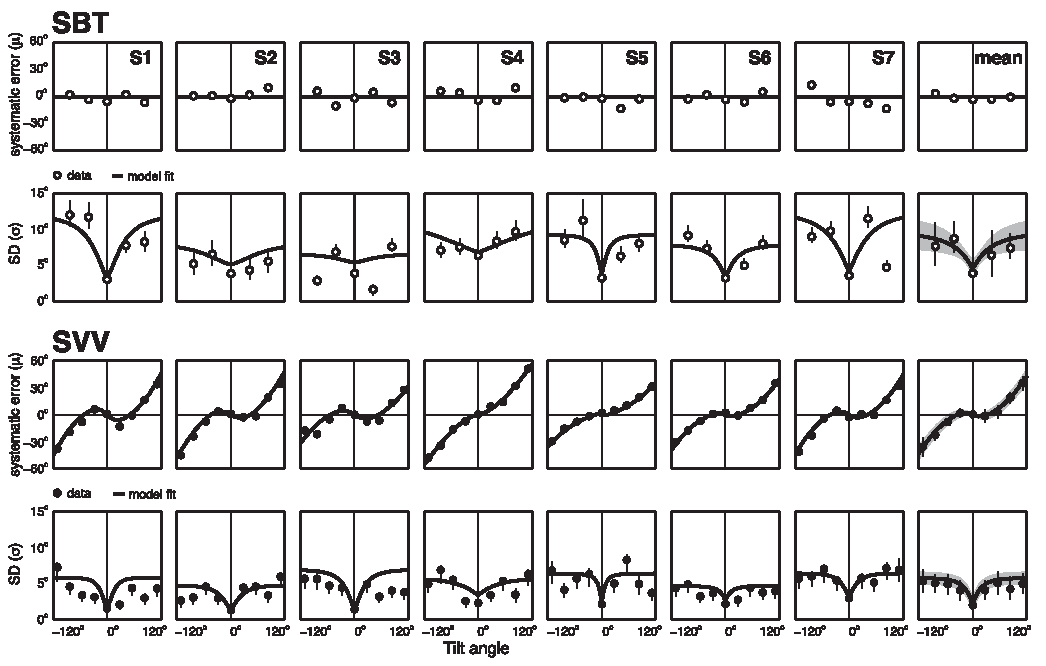
\includegraphics[width=1.0\textwidth]{src/paper1/figure4.pdf}
	
    \caption{Model predictions superimposed on parameters from the psychometric fits to the SBT (two top rows) and SVV data (two bottom rows). Accuracy and variability characteristics as a function of roll-tilt angle are shown; values are psychometric fits ($\mu$ and $\sigma$ values, $\circ$) and model predictions (line) from all subjects. Mean data and mean predictions across subjects are plotted in the rightmost column.}
    \label{p1:fig4}
\end{figure}

The two top rows in \figref{p1:fig4} show the accuracy ($\mu$) and precision ($\sigma$) of SBT percepts, now plotted against body orientation. For each subject, these values ($\mu$ and $\sigma$) were derived from the fitted cumulative Gaussian curves (\figref{p1:fig3}). Biases for SBT, shown in the top row of \figref{p1:fig4}, indicate moderate deviations in either direction from perfect performance, but no systematic pattern emerges. Across the seven subjects, the $\mu$ values ranged from \siang{-14.2} to \siang{+11.7} across the five SBT tasks. On average, however, there was no systematic bias for the five body orientations (ANOVA; F(4,24) = 1.4; $p = 0.25$), as also indicated by the rightmost panels. The data further show that, in all subjects, variability is statistically lower ($p < 0.05$) at the upright orientation, with $\sigma$ values \textless4\textdegree, than in the tilted conditions (\siang{45} and 90\textdegree), with $\sigma$ values ranging up to ~12\textdegree. 

The two bottom rows of \figref{p1:fig4} summarise our SVV data across the entire tilt range. Accuracy is close to perfect at upright orientation in all subjects, with mean values ranging between \siang{0.1} and 2.8\textdegree. For tilts $\ge60\degree$, all subjects show systematic SVV errors (biases) of undercompensation, ranging up to maximum values close to 60\textdegree. Three subjects (S1, S2, and S3) also show slight errors of overcompensation in the smallest tilt range (\textless60\textdegree). The variability in the SVV is \siang{\textless3.0} for upright, which is consistently lower than in the tilted conditions, where variability reaches values ranging up to 8\textdegree. 

Together, the results in \figref{p1:fig4} show that SVV and SBT have different accuracy and precision characteristics. Subjects perceive their body-tilt angle more accurately than the spatial orientation of the visual line. However, when it comes to variability, performance is reversed: SVV curves are narrower than the SBT curves in all subjects, at both tilt angles, meaning that they are consistently less variable in the SVV task than in the SBT task. 

\subsection{Model predictions}

The bold lines in \figref{p1:fig4} present the predictions of the Bayesian integration model, fitted simultaneously to the original responses from the SBT and SVV tasks. The rightmost column of \figref{p1:fig4} shows the mean predictions from this model superimposed on the averaged parameters from the psychometric fits, indicating that the sensory integration model can account very well for all the characteristics of the data. 

By design (see \nameref{p1:sec:methods}, the sensory integration model fits a horizontal fit line through $\mu_{SBT} = 0\degree$ because it cannot account for the small systematic SBT errors. As to SBT precision, the model predictions show an increase of noise with tilt angle similar to the actual increase of noise between \siang{0} and \siang{90} tilt, for all subjects. These model fits further suggest that the increase of SBT noise is steepest at small tilt angles and levels off at larger tilts. According to the model, the increase of SBT noise with tilt angle is attributable to the corresponding increase of noise in the head sensors (parameter $a_{HS}$), but levels off by the constant noise level in the body sensors. The third row in \figref{p1:fig4} depicts the model predictions of the systematic SVV errors, which show a very good match. Also with respect to SVV variability, fits and data show similar trends, suggesting an increase of SVV noise with tilt angle, which levels off at larger tilts. 

For each subject, best-fit parameter values and their bootstrap-based SD levels are listed in \tabref{p1:tab1}. Parameter $b_{HS}$, representing the noise ($\sigma_{HS}$) in the otolith signal in the upright subject, ranges between \siang{1.1} and \siang{3.9}. Best-fit values of parameter $a_{HS}$ are significantly positive ($p < 0.05$) for all subjects, ranging from \siang[/\degree]{0.07} (S4) to \siang[/\degree]{0.23} (S1). This implies that the noise in the otoliths increases with tilt angle. The width of the head-in-space prior ($\sigma_{HSP}$) ranges from \siang{9.4} (S2) to \siang{18.7} (S5), with a mean of 12.5 \textpm \siang{3.2}, consistent with our previous report \cite{devrijer2009}. Best-fit values of parameter $\sigma_{BS}$, reflecting the noise in the sensory body-in-space signal, range from \siang{6.7} (S3) to \siang{15.0} (S5), with a mean of 10.8 \textpm \siang{3.1}, which is about twice as large as the best-fit values of parameter $\sigma_{HB}$, reflecting noise in the head-on-body signal, ranging from \siang{1.8} (S6) to \siang{9.3} (S3), with a mean of 4.9 \textpm 2.7\textdegree. Thus, the parameter fits imply that the neck sensors are more precise than the body-tilt sensors. As has been discussed extensively in our previous paper \cite{devrijer2009}, the amplitude of uncompensated ocular counterroll ($A_{OCR}$) shows large inter-subject variability. 

\begin{table}

\begin{tabular}{lllllll}
\hline
Subject & $a_{HS}$ (\textdegree/\textdegree) & $b_{HS}$ (\textdegree) & $\sigma_{HSP}$ (\textdegree) & $\sigma_{BS}$ (\textdegree) & $\sigma_{HB}$ (\textdegree) & $A_{OCR}$ (\textdegree) \\
\hline
S1 & 0.23 \textpm 0.02 & 1.2 \textpm 0.32 & 11.6 \textpm 1.0 & 12.3 \textpm 1.1 & 3.3 \textpm 1.2 & 27.0 \textpm 2.2 \\
S2 & 0.12 \textpm 0.02 & 1.2 \textpm 0.52 & 9.4 \textpm 1.1 & 8.4 \textpm 2.9 & 6.4 \textpm 4.1 & 17.0 \textpm 3.8 \\
S3 & 0.20 \textpm 0.03 & 1.1 \textpm 0.42 & 14.4 \textpm 1.7 & 6.7 \textpm 1.9 & 9.3 \textpm 2.4 & 17.5 \textpm 2.1 \\
S4 & 0.07 \textpm 0.50 & 3.9 \textpm n/a & 11.2 \textpm 1.3 & 12.6 \textpm 2.3 & 7.1 \textpm 3.5 & 0 \textpm n/a \\
S5 & 0.11 \textpm n/a & 3.3 \textpm 1.0 & 18.7 \textpm 4.8 & 15.0 \textpm n/a & 3.6 \textpm 2.1 & 1.06 \textpm n/a \\
S6 & 0.23 \textpm 0.09 & 3.0 \textpm 1.5 & 9.5 \textpm 1.1 & 8.0 \textpm 0.83 & 1.8 \textpm n/a & 18.8 \textpm 4.1 \\
S7 & 0.20 \textpm 0.14 & 3.2 \textpm 1.0 & 12.8 \textpm 2.4 & 12.7 \textpm 6.1 & 3.0 \textpm n/a & 20.8 \textpm 9.0 \\
Mean & 0.16 \textpm 0.06 & 2.4 \textpm 1.2 & 12.5 \textpm 3.2 & 10.8 \textpm 3.1 & 4.9 \textpm 2.7 & 14.6 \textpm 10.2 \\
\end{tabular}

\caption{Best-fit parameter and bootstrap-based SD values. Imposed fit limits were as follows: $a_{HS}$: 0.5\textdegree/\textdegree; $b_{HS}$, $\sigma_{HSP}$, $\sigma_{BS}$, $\sigma_{HB}$, 50\textdegree; $A_{OCR}$, 30\textdegree. SD values are not shown (n/a) when bootstrapped values formed a skewed distribution. $a_{HS}$, Tilt-related increase in otolith noise; $b_{HS}$, otolith noise in upright position; $\sigma{HSP}$, width of head-tilt prior; $\sigma{BS}$, noise in body-in-space sensors; $\sigma{HB}$, noise in neck sensors; $A_{OCR}$, uncompensated ocular counterroll.}
\label{p1:tab1}
\end{table}

\subsection{Sensory weights}
 
To obtain the model fits in \figref{p1:fig4}, we made the assumption (see Introduction) that information from both direct and indirect pathways (\figref{p1:fig1}) is used to estimate body and head orientation in space. The sensory weights, indicating the relative contribution of both pathways, can be computed from the fit results in \tabref{p1:tab1}. To obtain the body-in-space estimate, necessary for the SBT, the model uses both direct information from the body sensors and indirect information from the combination of otolith and neck information. Because the variability of the otolith signal ($\sigma_{HS}$) increases with tilt angle ($a_{HS} > 0$), as shown in \tabref{p1:tab1}, the relative importance of direct and indirect pathways becomes dependent on tilt angle. This can be seen in \figref{p1:fig5} (top row), which shows the relative weights of these signals for each subject, derived from \eqnref{p1:eqn2} and the best-fit parameter values in \tabref{p1:tab1}. The mean (\textpm SD) pattern across subjects is shown in the rightmost pattern. 

\begin{figure}
    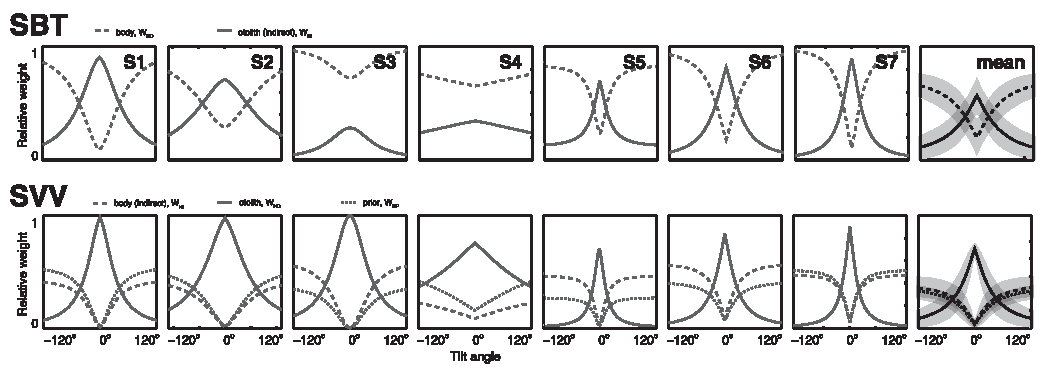
\includegraphics[width=1.0\textwidth]{src/paper1/figure5.pdf}
    
    \caption{Tilt dependence of weight factors in SBT (top) and SVV (bottom) for each subject. Trends with tilt angle are similar for all subjects. Head-in-space prior is only involved in SVV computations. Means across subjects are plotted in the rightmost column.}
    \label{p1:fig5}
\end{figure}

Instead of an overall dominance of body receptors in the direct pathway, the model implies that it is actually the indirect pathway, carrying the otolith signal, that dominates the behaviourally important range near upright. In most of our subjects (S1, S3, S5, S6, and S7), it was only when the otoliths became less reliable, at larger tilts, that the body sensors (direct pathway) got the upper hand ($w_{BD} > 0.5$). 

For the SVV task, the model assumes that both information from the otoliths (direct) and the combination of body and neck information (indirect) is used. \figref{p1:fig5} (bottom row) illustrates the relative contributions from these sensors as well as from the prior, based on the model fits (\tabref{p1:tab1}) and \eqnref{p1:eqn6}. The SVV pattern looks similar to the SBT pattern (\figref{p1:fig5}, top row): in all subjects, the otoliths are very dominant near upright, with weights close to 1, but their contribution declines when tilt angle increases. As we saw for the SBT signal weights, this decline reflects increasing otolith noise levels. In the SVV, the decline is steeper than in the SBT, where the reference frame transformation leads to an enhanced noise level with a less pronounced tilt dependence. As the otolith contribution decays, the contributions of the prior and indirect pathway become more manifest. According to our model fits, the weight of the body sensors in the SVV task ($w_{HI}$) at \siang{90} tilt ranges between 0.19 (S4) and 0.53 (S6). 

\subsection{Model evaluation}
 
To test whether the assumption of indirect pathways in the model is warranted, we compared its performance with a reduced version with only direct pathways (see \nameref{p1:sec:methods}). With this in mind, we performed a likelihood ratio test of the complete model fit (with direct and indirect pathways) versus the fit of a model with direct pathways only [i.e., SVV just based on head sensors (the otoliths), the SBT just based on body sensors]. The results are shown in \tabref{p1:tab2}. For each subject, the complete model provided a significantly better account of the data than the reduced model without multisensory integration through the indirect pathways. In other words, head, neck and body sensors all contribute to both SBT and SVV. 

\begin{table}
\begin{tabular}{llllll}
\hline
Subject & MLE full model & MLE reduced model & $p$ & BIC full model & BIC psychometric fits \\
\hline
S1 & 231.5 & 312.4 & \textless 0.001 & 498.1 & 540.3 \\
S2 & 197.8 & 216.9 & \textless 0.001 & 430.6 & 539.3 \\
S3 & 267.5 & 313.4 & \textless 0.001 & 570.0 & 548.2 \\
S4 & 207.5 & 218.2 & \textless 0.001 & 450.0 & 569.1 \\
S5 & 195.6 & 216.3 & \textless 0.001 & 426.2 & 571.0 \\
S6 & 163.5 & 183.2 & \textless 0.001 & 362.0 & 502.5 \\
S7 & 248.0 & 260.0 & \textless 0.001 & 531.1 & 633.5 \\ 
\end{tabular}
\caption{Validation of the model. Log-likelihood ratio test of the full model (with indirect pathways) and reduced model (without indirect pathways). For all subjects, the full model outperforms the reduced model lacking multisensory integration through the indirect pathways. BIC values are much lower for the Bayesian integration model compared with separate psychometric fits in six of seven subjects.}
\label{p1:tab2}
\end{table}

We also compared our model, which provides a mechanistic explanation of the full dataset, with the pure descriptive account of the data as obtained by fitting separate psychometric curves to the data for the five SBT angles and nine SVV angles (\eqnref{p1:eqn1}, \figref{p1:fig3}, and \nameref{p1:sec:methods}, Model evaluation). Maximum-likelihood estimates were calculated and corrected for the number of free parameters using the BIC. As shown in \tabref{p1:tab2}, we found the lowest BIC values, indicating a better model, for the Bayesian model in all subjects, except S3. One might argue that the mean corrections before fitting the Bayesian model added another nine parameters that should be taken into account when comparing the models, even though these parameters were not fitted by the model. However, even for the worst-case scenario of 16 parameters, our Bayesian model still outperformed the individual psychometric fits ($\text{BIC}_\text{mechanistic} = 3583 < \text{BIC}_\text{psychometric} = \text{3910}$). 

\subsection{Model validation}
 
To further validate the model, we independently tested one of its predictions that can be assessed experimentally in isolation: head-on-body variance. In supine position, subjects judged their head orientation (CW/CCW) relative to the body midline after it had been passively roll-rotated with speeds subthreshold for the canals to various angles (see \nameref{p1:sec:methods}, Model validation: independent test of neck noise). Psychometric fits indicate no systematic bias in these head-on-body percepts (data not shown). Figure \ref{p1:fig6} depicts the experimental noise levels derived from these psychometric fits and the predicted values provided by the model, including their 95\% confidence intervals. Because the variance of the estimates increases with the average head-on-body percept, we performed a regression on the log-transformed data \cite{hopkins2000}. The significant correlation between predicted and measured neck noise levels (slope, 1.03; intercept, -0.1; $p = 0.04$) provides an independent confirmation of the proposed model.

\begin{SCfigure}
    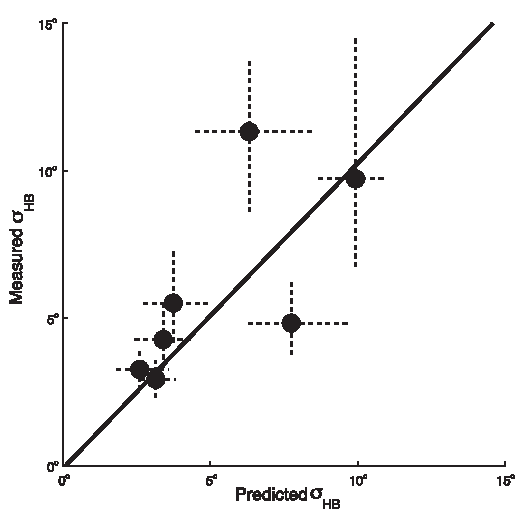
\includegraphics[width=0.35\textwidth]{src/paper1/figure6.pdf}
    
    \caption{Model validation. Independent measurement of neck (head-on-body) noise ver- sus the values predicted by the model. The dots represent the median values and the dashed lines the 95\% confidence interval determined from a bootstrap. Note that the variance of the estimates increases with the mean value. The solid line shows the regression based on log-transformed data (slope, 1.03; $p = 0.04$).}

    \label{p1:fig6}
\end{SCfigure}


%%%%%%%%%%%%%%
% Discussion %
%%%%%%%%%%%%%%

\section{Discussion}

In this study, we made intra-subject comparisons of the accuracy (bias) and precision (inverse variance) characteristics in two spatial orientation tasks: SBT and SVV. The main experimental findings were as follows: (1) the SBT is more accurate than the SVV, (2) the SBT is less precise than the SVV, and (3) both SBT and SVV precision are smaller in tilted conditions than near upright. Under the assumption of optimality, a Bayesian model of sensory integration could account very well for these findings. Independent measurements, in supine subjects, of head-on-body variance confirmed the predicted value. 


\subsection{Comparison with previous work}
 
A world-vertical visual line appears tilted in space when the head is tilted in a darkened room \cite{aubert1861}. Mittelstaedt \citeyear{mittelstaedt1983} was the first to emphasise that this phenomenon cannot be explained by errors in the body-tilt percept. He showed that subjects could accurately adjust themselves to a horizontal position, but, once in this position, made substantial systematic errors in the perception of visual verticality. Later, combined tests confirmed the discrepancy between SVV and SBT accuracy \cite{mast1996, jarchow1999, vanbeuzekom2000, vanbeuzekom2001, kaptein2004, vingerhoets2008}. The present study is consistent with these findings, showing substantial systematic SVV errors at tilts $\ge60\degree$ and fairly accurate SBT performance. 

Compared with the abundant literature on SBT and SVV accuracy, data on their perceptual variability are scarce. In contrast to Mittelstaedt's observation \citeyear{mittelstaedt1983}, Mast and Jarchow \citeyear{mast1996} found that the SBT was much more variable than the SVV. The present study, the first to measure both SVV and SBT precision using an extensive psychometric approach, has clearly established that SBT variability is consistently higher than SVV variability, both in the upright and in the horizontal (90\textdegree) tilt position. 

Furthermore, although various studies have noted that SVV variability increased at larger tilts \cite{schone1964, schone1968, udodehaes1970, vanbeuzekom2001, devrijer2008}, little is known about SBT variability as a function of tilt angle. Nelson \citeyear{nelson1968} showed that subjects were more variable when adjusting themselves to a horizontal position than to a vertical (upright) position. The present findings are consistent with these early observations. 


\subsection{Implications of the model}
 
After earlier indications that both the otoliths and body sensors contribute to the SBT \cite{clark1963, clark1964, nelson1968}, Mittelstaedt \citeyear{mittelstaedt1997} made a quantitative assessment of their impact, using an ingeniously designed experiment. Subjects lay on their side in a horizontal centrifuge. The crux of the experiment was to vary the distance between the rotation axis and the interaural axis to equalise the opposite contributions from the otoliths and the body sensors so that the subject felt horizontal. By testing normal, paraplegic, and nephrectomised subjects, Mittelstaedt inferred how much each sensory system contributes to body-tilt perception. It was shown that, apart from the otoliths, also internal ``graviceptors'' in the trunk (such as the viscera) participate in the computation of the SBT. Later, some related studies provided evidence that the distribution of blood in the body also affects postural perception \cite{vaitl1997, vaitl2002}. According to Mittelstaedt \citeyear{mittelstaedt1998}, the weight of the somatic graviceptors to estimate horizontal body orientation in healthy subjects is \textapprox0.6 on average, with considerable inter-subject variability. His estimate seems quite compatible with our $w_{BD}$ values at \siang{90} tilt, which range between 0.35 (S5) and 0.93 (S6) (\figref{p1:fig5}). 

Previous attempts to identify the separate contributions of the otoliths, neck, and body sensors on the SVV have yielded mixed results. Whereas Mittelstaedt \citeyear{mittelstaedt1998} found no evidence that the SVV was affected by the body sensors in his centrifuge experiment, other studies indicate that neck- and trunk-tilt aftereffects \cite{wade1968}, neck muscle vibration \cite{mckenna2004}, and manipulation of tactile and interoceptive body cues \cite{trousselard2004} can affect the SVV. In other words, even in the absence of direct head-in-space information from the otoliths, the brain can still obtain an estimate of head orientation in space through the indirect sensory pathway. These findings suggest that these modalities operate together with the otoliths in the computation of the SVV, consistent with our model. 


\subsection{Model evaluation}
 
The architecture of the model, as far as the reference frame transformations and the sensory integration is concerned, follows entirely from the principles of Bayesian inference. However, to account for our major findings and inter-subject differences, we made two less straightforward assumptions. First, to explain the increased variability in both tasks at \siang{90} tilt, we allowed for the possibility that the otoliths become more noisy with increases in tilt. Second, we hypothesised that prior knowledge is used in the visual vertical but not in body-tilt perception. Can these assumptions be justified on physiological and rational grounds? 

One reason to assume that otolith noise depends on tilt angle is based on the fact that the utricle contains considerably more hair cells than the saccule \cite{rosenhall1972, rosenhall1974}. Because the utricle is most sensitive to tilts of \textapprox0\textdegree, whereas the saccule is most sensitive at \siang{\textapprox90} tilt \cite{jaeger2008}, this may well cause the proposed increase of otolith noise with tilt angle \cite{tarnutzer2010}. A tilt-dependent noise level of the otoliths would also help to explain why the perturbing effect of roll-optokinetic stimulation on the SVV \cite{dichgans1974, fernandez1976} and on the SBT \cite{young1975} is more pronounced at larger tilt angles and why the SVV is more strongly influenced by residual canal signals at larger tilt angles, after prolonged roll rotations \cite{lorincz2008}.

In the SVV literature, it is widely assumed that the visual vertical is determined by a weighted combination of a sensory head-tilt signal and a head-fixed reference, denoted as the idiotropic vector \cite{mittelstaedt1983}. Recently, this idiotropic vector has been reinterpreted in terms of a Bayesian prior \cite{eggert1998, macneilage2007, devrijer2008}, with which it is mathematically equivalent. Interestingly, when tested in gravity-free conditions, subjects still retain a sense of visual vertical, always aligned with their long-body axis, compatible with the idea of head-fixed prior \cite{mittelstaedt1983}. Vingerhoets et al. \citeyear{vingerhoets2008} recently found a similar phenomenon in the SVV during multiple-cycle dynamic roll rotation in normal gravity. Remarkably, when the same subjects were tested in a comparable dynamic SBT experiment, their responses showed very little bias on average, indicating that a prior is used only in the SVV and not for body-tilt estimation. To explain how this difference in computational approach might make sense, Vingerhoets et al. \citeyear{vingerhoets2008} speculated that precision is more important than accuracy for the visual system, for reasons of visual stability. Combining the sensory tilt signal with prior knowledge yields a more stable percept of visual space than can be derived from the sensory signal alone. In a recent study, Bortolami et al. \citeyear{bortolami2006} report virtually no bias in the haptically indicated vertical, which would be consistent with the suggestion that the prior plays primarily a role in visual processing. Likewise, for body-tilt perception, for which it might be less important to be precise and more useful to be accurate, the prior does not take part in this process. 

\subsection{Clinical implications}
 
According to our model, statistically optimal performance requires the use of information from both direct and indirect pathways to estimate body and head orientation in space (\figref{p1:fig1}). Thus, if one of the sensory inputs is lost or severely disrupted, SBT and SVV performance will deteriorate, but should not completely break down due to their multimodality dependence. By setting the appropriate parameter values of the model to infinity, we simulated the model to predict SVV and SBT performance in two patient groups: bilateral vestibular patients (noise level of the otoliths set to infinity) and patients with somatosensory loss (noise level of the body sensors set to infinity). \figref{p1:fig7} shows the results of these simulations. 

% FIXME: Change figure 7 such that the panels are side-by-side.
\begin{SCfigure}
    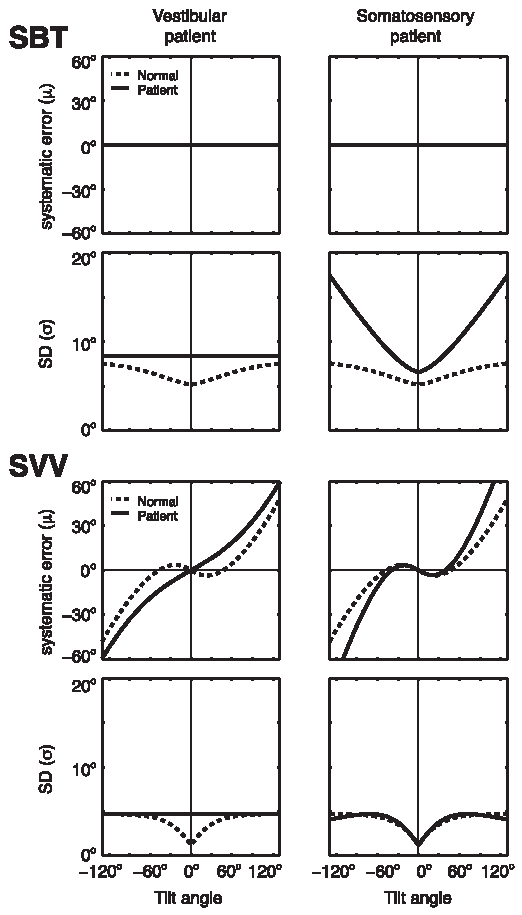
\includegraphics[width=0.5\textwidth]{src/paper1/figure7.pdf}
    
    \caption{Clinical implications of the model. The model simulates the SBT and SVV in a vestibular patient by raising the level of the otolith noise to infinity, keeping the other parameters at the mean values of \tabref{p1:tab1}. A somatosensory patient is modelled by setting the noise level of the body sensors to infinity. Solid lines, Patient predictions. Dashed lines, Prediction for normals.}
    \label{p1:fig7}
\end{SCfigure}

When the otolith signal is lost (vestibular patient), the model predicts increased but constant noise levels in both the SBT and SVV, regardless of tilt angle. From the perspective of our model, the increased SBT variability can be attributed to the loss of the otolith contribution through the indirect body-in-space pathway. The increased bias in the SVV, predicted by the model, can also be understood: as the sensory-derived head-tilt estimate becomes noisier, the effect of the prior becomes more noticeable. Although there are no accuracy and variance measurements across the entire tilt range in these patients, the few previously published deficits are consistent with these predictions. Bisdorff et al. \citeyear{bisdorff1996} have shown that bilateral vestibular patients performed quite accurately in the SBT at upright, but were \textapprox40\% more variable than normal subjects. Bronstein et al. \citeyear{bronstein1996} showed that vestibular patients still compensated for their tilt angle when testing the SVV at 90\textdegree, but with a bias about twice as large as in normal subjects, consistent with our simulations. 

The right column of \figref{p1:fig7} depicts a simulation of the SBT and SVV in a patient with loss of somatosensory information (somatosensory patient). In this case, the SBT depends solely on otolith information mediated through the indirect pathway. Although this signal is still accurate, it is spoiled by the larger variability of the neck signal, needed to perform the appropriate reference frame transformation. The model also predicts larger errors in the SVV in these patients than in normal subjects. Although there are no reports containing measurements of bias and variance in the SBT and SVV, paraplegic patients show that along with the otoliths, internal body sensors also contribute to the SBT if lesions are below the 12th thoracic segment \cite{mittelstaedt1997}. This evidence supports the design of our model. 

In conclusion, we have tested the performance of healthy subjects in two psychophysical tasks that probe two spatial orientation estimates (SBT and SVV) and show that perceptual accuracy and precision in these tasks can be linked to the reference-frame-dependent weighting of sensory signals. We verified our theoretical framework by independent measurements of neck noise levels and by showing that it can account for the stereotypical performance of two patient groups. In this respect, our reverse-engineering approach also provides a new tool to establish diagnostic and prognostic markers of the quality of the signals involved in spatial orientation in neurological disease. 


%%%%%%%%%%%%
% Appendix %
%%%%%%%%%%%%

\section{Appendix}
\label{p1:sec:appendix}

Here we provide further explanation about the Bayesian computations underlying the SVV as expressed in \eqnref[ and ]{p1:eqn6,p1:eqn10} in Materials and Methods. \figref{p1:fig8} illustrates graphically that the variance of the posterior distribution in a single trial ($\sigma^2_{\tilde{H}S}$) is not simply the same as the variance in its peak location in multiple trials, $\sigma^2(\tilde{H}_S)$. In a single trial (\panelref{p1:fig8}{A-C}), the optimal estimate of head tilt is based on the likelihood (\figref{p1:fig8}B, green curve) associated with the combined sensory input from the direct and the indirect pathway (\panelref{p1:fig8}{A}, green line, $\hat{H}_S$) and the prior (\panelref{p1:fig8}{B}, blue curve), by multiplication of the two probability distributions. The prior distribution is a Gaussian with mean $H_{SP}$ and variance $\sigma^2_{HSP}$. The peak of the resulting posterior distribution (\panelref{p1:fig8}{B-C}, orange curve) is used as the optimal estimate of head tilt ($\tilde{H}_S$), given by the following: 

% Equation 13
\begin{equation}
\label{p1:eqn13}
\tilde{H}_S = w_{HS} \cdot \hat{H}_S + w_{HP} \cdot H_{SP},
\end{equation}

with

% Equation 14
\begin{equation}
\label{p1:eqn14}
w_{HS} = \frac{1 / \sigma^2_{HS}}{1 / \sigma^2_{HS} + 1 / \sigma^2_{HSP}},
\end{equation}

and

% Equation 15
\begin{equation}
\label{p1:eqn15}
w_{HP} = \frac{1 / \sigma^2_{HSP}}{1 / \sigma^2_{HS} + 1 / \sigma^2_{HSP}},
\end{equation}

in which $\sigma_{HS}$ denotes the noise in the sensory signal, known to the observer, and $w_{HS}$ and $w_{HP}$ represent the relative weights of the sensory signal and the prior, respectively. Note that \eqnref{p1:eqn13} is equivalent to \eqnref{p1:eqn1} in \nameref{p1:sec:methods}. The variance of the posterior distribution in a single trial is given by the following: 

% Equation 16
\begin{equation}
\label{p1:eqn16}
\sigma^2_{HS} = w_{HS} \cdot \sigma^2_{HS} \\
              = \frac{\sigma^2_{HSP}}{\sigma^2_{HS} + \sigma^2_{HSP}} \cdot \sigma^2_{HS}
\end{equation}

and is reflected by the width of the orange curve in \panelref{p1:fig8}{B}. \panelref{p1:fig8}{D-F} illustrates performance in multiple trials, in which the posterior distributions vary due to sensory noise ($\sigma_{HS}$), whereas the prior remains fixed. The variance of each posterior distribution is fixed and is given by \eqnref{p1:eqn16}. 

\begin{figure}
    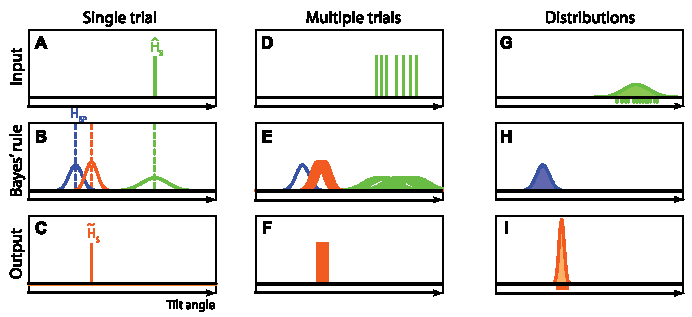
\includegraphics[width=0.80\textwidth]{src/paper1/figure8.pdf}
    \caption{Bayesian computations in single and multiple trials. A-C, Single trial. D-F, Multiple trials. G-I, Resulting distributions. For further explanation, see \nameref{p1:sec:appendix}.}
    \label{p1:fig8}
\end{figure}

That the variance of the peak locations across multiple trials, $\sigma^2(\tilde{H}_S)$, is smaller can be shown by applying the rules of noise propagation to \eqnref{p1:eqn13}. 

% Equation 17
\begin{equation}
\label{p1:eqn17}
\sigma^2(\tilde{H}_S) = \\
	\big( \frac{\delta\tilde{H}_S}{\delta\hat{H}_S^2} \big) \cdot \\
	\sigma^2(\hat{H}_S) + \\
	\big( \frac{\delta\tilde{H}_S}{\delta H_{SP}^2} \big) \cdot \\
	\sigma^2(H_{SP}) \\
	= w^2_{HS} \cdot \sigma^2_{HS} \\
	= \frac{\sigma^2_{HSP}}{\sigma^2_{HS} + \sigma^2_{HSP}} \cdot \sigma^2_{HS}
\end{equation}

which is equivalent to \eqnref{p1:eqn10} in Materials and Methods. Corresponding panels G-I (\figref{p1:fig8}) illustrate the distribution of the sensory signals for a given tilt angle (green-shaded curve), the prior distribution (blue-shaded curve), and the optimal estimates (orange-shaded curve), respectively. \panelref{p1:fig8}{I} illustrates that the distribution of the optimal estimates across many trials has a lower variance than the posterior distribution in each single trial (\panelref{p1:fig8}{B}), which follows from the comparison of \eqnref{p1:eqn16,p1:eqn17}, respectively. 

